\begin{figure*}[t]
    \centering
    \vspace{-20pt}
    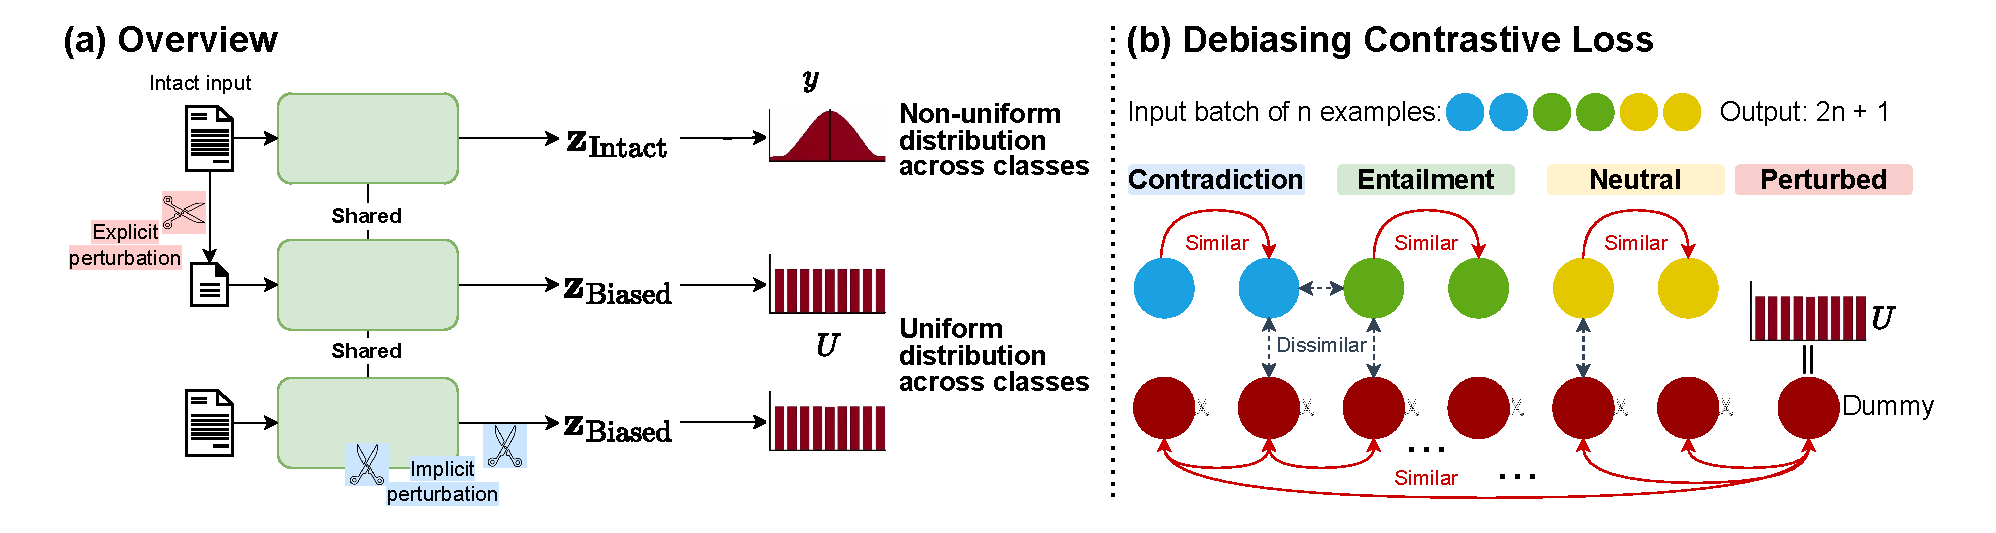
\includegraphics[width=.9\textwidth]{figure/fairflow.pdf}
    % \vspace{-20pt}
    \caption{Architecture of the proposed model. (a) Explicit and implicit perturbations are applied to inputs to obtain biased prediction $z_{\mathrm{Biased}}$. (b) Biased predictions are drawn closer to uniform distribution, while predictions for intact input are pushed away from uniform distribution through contrastive learning.}
    \label{fig:model}
    % \vspace{-10pt}
\end{figure*}

\section{Method}
\subsection{Problem Formulation}
We consider a dataset $\mathcal{D} = \{(x_i, y_i)|_{i=1}^n\}$, where $x_i$ is the $i$-th input consisting of several constituents $x_i = (x_i^1, x_i^2, \dots, x_i^p), |x_i| = p > 1$, and $y_i$ is the corresponding output for $x_i$. For example, in case of NLI, $p=2$ represents premise and hypothesis in each input and $y_i$ reflects the entailment or no-entailment relationship between the input pair. Our goal is to develop a model that is robust against different types of dataset biases in $\mathcal{D}$. 
We note that the model can be applied to a more general setting where input $x_i$ does not explicitly consist of several constituents, see \S\ref{sec:explicit_bias}.

% \subsection{A Motivating Example}
% As Figure~\ref{fig:motivating_example} shows, when given an intact premise-hypothesis pair, we want to train an NLI model to be determined about the label, since the input contains full information about the relationship between the input pair. However, if the input only contains the premise, the model should not be able to infer any information about the relationship between the premise and the hypothesis, because the hypothesis is missing. Even though the premise itself is still a valid sentence, it does not allude any signal about its relationship with another absent sentence. If a model is still confident about a label given partial input, it is very like that it relies on shortcuts to make predictions. Therefore, given such \textit{significantly corrupted instances or representations}, a robust model should remain \textit{undecided about the label}, encouraging itself to focus on causal signals rather than spurious shortcuts.


\subsection{Overview}
We categorize dataset biases as \textit{explicit} and \textit{implicit} biases. Explicit biases are readily discernible and understandable by humans, such as high degree of lexical overlap between the premise and hypothesis in case of NLI. On the other hand, implicit biases are often subtle, indiscernible to humans, and more challenging  
%linguistic (lexical or syntactic) 
% characteristics are unknown
to detect. For example, any word in input has the potential to act a shortcut, resulting in spurious correlations. 
We introduce different types of explicit and implicit biases that are {\em task-independent} and generally applicable to bias mitigation across NLP datasets (\S\ref{sec:biasmodeling}). 
%
Given such categorization, we propose a debiasing framework that mitigates dataset biases by learning genuine task-related representations that are attentive to the true signal of the tasks rather than biases and shortcut solutions in datasets. 
The key novelty of our approach is in imposing a downstream model to adopt an ``undecided'' (``uncertain'') stance in its predictions when presented with biased views of inputs. The framework achieves this goal by assigning a uniform probability across the labels, see \textbf{Figure~\ref{fig:model}}. 
Specifically, the model regularizes the loss of the target task with a contrastive loss which draws biased predictions closer to a uniform distribution while pushing other predictions away from uniform distribution (\S\ref{sec:contrastive}).  
%



% \paragraph{Bias Categorization}

% \hadi{explain/justify why each type should be considered for debiasing and how it contributes to debiasing.}

% . Some are not human perceivable. We term these biases as implicit biases. In addition to the above explicit biases, there exist other types of biases that are not as explicit as lexical or subpart bias. Other types of biases may be hard to categorize. 

% \subsubsection{Explicit Biases}
% \paragraph{Sub-input bias (explicit)} 



\subsection{Bias Modeling}\label{sec:biasmodeling}
We present a series of data perturbation operations to generate biased views by corrupting intact inputs. These perturbations can be explicit or implicit. In explicit perturbation, we directly corrupt the input data, while in implicit perturbation, we corrupt the representations of the input data. These perturbation techniques impose controlled variations on the data, which enable us to conduct a thorough analysis of their effects on bias mitigation.



% We first propose a set of data perturbations that explicitly perturb the input data. Then we model the biases in these explicitly perturbed data to force our model to make uniform predictions. We consider several types of known biases: 

\subsubsection{Explicit Biases} \label{sec:explicit_bias}
% We introduce Sub-input and Ungrammatical explicit perturbations. 

% \hadi{re lexical overlap and negation perturbations: these are tasks specific.. also, our stress sets includes these.. so our eval won't be fair as we are directly optimizing on biases that we know exist in test sets. }

% we propose a set of data perturbation operations that explicitly perturb the input data. Then we model the biases in these explicitly perturbed data and force our model to make uniform predictions.
\paragraph{Ungrammatical Perturbation} Recently, \citet{sinha-etal-2021-unnatural} showed that traditional and recent neural language models can be largely invariant to random word order permutation in their inputs. 
An ungrammatical input is often not understandable by humans and can potentially lead to explicit biases when models confidently predict outcomes for such inputs. For example, a model making a confident prediction about the contradiction class for the following perturbed premise-hypothesis pair from Figure~\ref{fig:example} may attribute its confidence to the negation term in the hypothesis: (``{\tt children fun for}'', ``{\tt children fun adults but for not}''). 
% premise: (``{\tt children fun adults but for not}'', ``{\tt children only for fun}''). 
To obtain an input with grammatical biases, we design the perturbation operation $\mathcal{P}_{Gra}$ that 
% randomly shuffles 
corrupts the word order in each input $x_i$. We encode the shuffled input using the shared encoder $f$ and transform it with a branch-specific MLP as follows:
\begin{equation}
    z_{Gra} = \texttt{MLP}_{Gra} \Big( f\big(\mathcal{P}_{Gra}(x_i) \big) \Big).
\end{equation}


\paragraph{Sub-input Perturbation} 
In NLP tasks that involve multi-part inputs (such as NLI), it is crucial to use the information from all parts of the input for prediction, i.e., all constituents should collectively contribute to accurate prediction. More importantly, an incomplete input should not lead to a confident prediction, as important information may be removed. 
Therefore, an explicit bias arises when the model makes confident predictions based on incomplete input, such as predicting the \textit{entailment} relation when only the hypothesis is provided as input in case of NLI. Sub-input biases can arise from any part of the input, denoted as $\{x_i^j\}_{j=1}^p$, or from various text spans within different sub-parts.
To realize sub-input biases, we define the $\mathcal{P}_{Sub}$ operator that takes one of the constituents of $x_i$, which is hen encoded with a shared encoder $f$ and further transferred with a constituent-specific $\texttt{MLP}_{Sub}$ as follows:
\begin{equation}
\label{eq:sub_aug}
    z_{Sub} = \texttt{MLP}_{Sub}\Big( f\big (\mathcal{P}_{Sub}(x_i)\big) \Big).
\end{equation}

\noindent We note that this operator is applicable to a more general setting where input $x_i$ does not explicitly consist of several constituents, e.g., in general text classification problems. In such cases, each $x_i$ can be divided into $p>1$ text segments. However, we acknowledge that there are tasks in which one sub-input, i.e. ${x_i^j}$ for a specific $j$, is enough to make a correct prediction for the complete input ${x_i}$, and therefore remaining undecided may seem counter-intuitive. Nevertheless, by training the model to be undecided when presented with incomplete information, we minimize the risk of biased predictions based solely on partial information, which can, in turn, make the model more robust against potential biases associated with incomplete data. 


% \paragraph{Lexical Overlap Perturbation} 
% \paragraph{Irrelevant Text Perturbation} 
% Deep learning models are vulnerable to wording of their inputs~\citep{gururangan-etal-2018-annotation}. In fact, they may focus on specific keywords and ignore the semantic and syntax analysis that is often required to effectively process the text. To obtain an input with irrelevant text biases, we design the perturbation operation $\mathcal{P}_{Irr}$  that appends irrelevant text to all the constituents of $x^i$. We encode the perturbed input using the shared encoder $f$ and transform it with a branch-specific MLP as follows:
% \begin{equation}
%     z_{Irr} = \texttt{MLP}_{Irr} \Big( f\big(\mathcal{P}_{Irr}(x_i)\big) \Big).
% \end{equation}

% \paragraph{Negation perturbation} Specific input words can have superficial correlations with labels, such as negation words in hypothesis in case of NLI. Models are prone to focus only on such superficial correlations, ignoring information from other parts. For example, BERT tends to classify examples as \textit{contradictory} because of the negation words in the hypothesis, neglecting the entailing relation between the premise and the hypothesis~\citep{karimi-mahabadi-etal-2020-end}. %Unlike previous works~\citep{}, 
% To obtain an input with negation bias, we design an perturbation operation $\mathcal{P}_{Neg}(\cdot)$ that adds negation words to the input $x^i$ as an perturbation. We encode the perturbed input using the shared encoder $f$ and transform it with a branch-specific MLP following 
% \begin{equation}
%     z_{Neg} = \texttt{MLP}_{Neg} \Big(f\big(\mathcal{P}_{Neg}(x^i)\big)\Big).
% \end{equation}


\subsubsection{Implicit Biases}
\label{sec:imp_bias}
The idea of implicit perturbations is to obtain biased representations of intact data, without explicitly perturbing the input. We introduce model- and representation-based implicit perturbation.

\paragraph{Model-based Perturbation} This approach largely perturbs a given model by converting it into a much weaker model, using mechanisms such as sparsification and layer dropping~\citep{NEURIPS2021_6e8404c3}. A weaker model is believed to capture more biases than a stronger model~\citep{ghaddar-etal-2021-end,sanh2020learning,utama-etal-2020-towards}. While existing methods require training a weak learner in advance~\citep{utama-etal-2020-towards,sanh2020learning,meissner-etal-2022-debiasing}, our method obtains biased predictions through the same deep neural model ($f$) and can be trained \emph{end-to-end}. Formally, we design a model-based perturbation operator $\mathcal{P}_{Mod}$ that uses only the first $k$ layers of the shared encoder $f$, which results in a substantially weakened model with reduced representation power. This branch encodes the intact input using the perturbed model and transform it with a branch-specific MLP as follows:
\begin{equation}
    z_{Mod} = \texttt{MLP}_{Mod} \Big( \mathcal{P}_{Mod}(f)(x_i) \Big).
\end{equation}



\paragraph{Representation-based Perturbation} This perturbation encodes the intact input with the original encoder $f$ but significantly corrupts the generated representations. Given this severely damaged and much less meaningful representation, the model should not be able to predict the correct label. We design a representation-based perturbation operator $\mathcal{P}_{Rep}$ that corrupts the intact representation, $f(x_i)$, and creates a severely perturbed representation. We then transform the perturbed representation with a branch-specific MLP as follows:
\begin{equation}
\label{eq:rep_aug}
    z_{Rep} = \texttt{MLP}_{Rep} \Big( \mathcal{P}_{Rep} \big( f(x_i) \big) \Big).
\end{equation}


% either modeling the existing biases or creating additional biases. 



% \paragraph{Perturbation}
\textbf{Table~\ref{tab:aug_list}} summarizes the above perturbation operators and provides details of their implementations. 
% DropPremise, which drops the premise part of the input; 2) DropHypothesis, which drops the hypothesis part of the input; 3) HalfHalf, which randomly takes 50\% of the tokens from each sentence; 4) Shuffle, which randomly shuffles the premise and the hypothesis; 5) DropLayer, which drops all layers after the 2nd layer; and 6) DestroyRep, which zeros out 90\% of the elements in the intact representation.




\subsection{Supervised Contrastive Debiasing}\label{sec:contrastive}
Given the explicit and implicit biased views of data samples, we expect a robust debiasing model to maintain an ``undecided'' stance across labels for biased inputs while providing confident predictions for intact inputs $x_i, \forall i$. Based on this intuition, the outputs of the bias branches should approximate a {\em uniform distribution} ($U$) across classes, while the output of the original branch should align with its corresponding gold distribution, i.e., the label $y_i$. 
% Through back-propagation, we can achieve the goal of debiasing the representations of the backbone model. 
To achieve this goal, we adapt the supervised contrastive loss~\citep{khosla2020supervised}, which operates by first grouping samples based on their respective labels, and then encouraging predictions (logits) of pairs within the same group to become closer while pushing logits of pairs across different groups further apart, i.e. forming positive pairs within the same group while creating negative pairs using all other pairs: % (see footnote 2).
% i.e. forming positive pairs within the same group while creating negative pairs across different groups.

\begin{table}\small
\centering
\setlength{\tabcolsep}{3pt}
\renewcommand{\arraystretch}{1} 
\begin{tabular}{c|c|l}
\toprule
\textbf{Operator}               & \textbf{Type}     & \textbf{Implementation} \\
\midrule
$\mathcal{P}_{Gra}$ & Explicit & Shuffle tokens in $x_i$ randomly \\
$\mathcal{P}_{Sub}$  & Explicit & Drop $1/p$ of tokens from $x_i^j$ randomly \\
$\mathcal{P}_{Sub}$  & Explicit & Drop $x_i^j, j=1\dots p$ \\
% $\mathcal{P}_{Irr}$  & Explicit & Add same irrelevant text to all $x_i^j$ \\
% $\mathcal{P}_{Neg}$  & Explicit & Add negation words to all $x^i_p$ \\
\midrule
$\mathcal{P}_{Mod}$  & Implicit & Use only first $k$ of layers of $f$\\
$\mathcal{P}_{Rep}$  & Implicit & Zero out $m\%$ of values in $f(x_i)$ \\
\bottomrule
  \end{tabular}
  \caption{Implementations of proposed perturbations}
  \label{tab:aug_list}
  \vspace{-10pt}
\end{table}


We adapt this loss function for bias mitigation as follows (described for a single perturbation for simplicity):
given a batch of $n$ non-perturbed examples, we perturb them using a perturbation technique described in Table~\ref{tab:aug_list}. The perturbed examples form a single group as they all have the same label (a uniform distribution across all classes), and the non-perturbed examples with the same label form separate groups.\footnote{For example, four groups in case of NLI: perturbed examples, non-perturbed examples labeled as `entailment', non-perturbed examples labeled as `contradiction', and non-perturbed examples labeled as `neutral'.} 
As illustrated in \textbf{Figure~\ref{fig:model}}, we encourage the model to be undecided about the label of perturbed inputs by adding a dummy example that has a ``fixed'' uniform distribution across all labels to the group of perturbed examples, resulting in a batch of $2n+1$ examples ($\mathcal{I}$). We compute the contrastive loss as follows:
\begin{multline}
\label{eq:supcontras}
    \mathcal{L}_{\mathrm{Debias}} = \\ 
    \sum_{i \in \mathcal{I}} \frac{-1}{|\mathcal{G}(i)|} \sum_{j \in \mathcal{G}(i)} \mathrm{log} \frac{\mathrm{exp} (z_i \cdot z_j / \tau)}{\sum_{k \in \mathcal{A}(i)} \mathrm{exp} (z_i \cdot z_k / \tau)},
\end{multline}
where $\mathcal{G}(i)$ is the set of examples that are in the same group as $i$ (having the same label as $i$); 
$\mathcal{A}(i) = \mathcal{I}\backslash\{i\}$ is the set of all examples except $i$; 
$z$ indicates the logit of an example, which for perturbed examples is obtained from one of the Equations (\ref{eq:sub_aug})--(\ref{eq:rep_aug}); and 
$\tau$ denotes the temperature parameter.\footnote{We note that the summation over all samples except $i$ in the denominator of (\ref{eq:supcontras}) is motivated by noise contrastive estimation and N-pair losses~\citep{khosla2020supervised,pmlr-v9-gutmann10a,NIPS2016_6b180037}, in which the ability to discriminate between signal and noise (negative class) is improved by adding more examples of negative class.} The dummy example in the perturbed group has a fixed uniform distribution across all labels as its $z$. This formulation encourages the model to be undecided about the label of perturbed inputs, while being confident about the labels of intact inputs, allowing it to effectively distinguish between different groups of examples. 

% Given the logit of each example non-perturbed example $z_i$ from Equations \ref{eq:sub_aug}--\ref{eq:rep_aug}, ee enforce $z_{2N+1}$ to be a ``fixed'' uniform distribution across all labels, which can be thought of as adding a dummy example of uniform distribution to the group of perturbed examples. This dummy example is used for creating positive pairs for examples within the perturbed group. This adjustment enables the model to learn representations that can effectively distinguish between perturbed and non-perturbed examples. Given an index $i$, $G(i)$ denotes the indices in $I$ from the same group of $i$. The contrastive debiasing loss is defined as % If the $i$-th example is non-perturbed, $P(i)$ denotes the indices of the examples whose labels are the same as $i$'s. If the $i$-th example is perturbed, $P(i)$ denotes the indices of uniform distribution. We enforce the logits $z_p$ in the numerator of Eq.~\ref{eq:supcontras} 



% $A(i) = I\backslash\{i\}$ and $\tau$ denotes the temperature parameter. This formulation encourages the model to be undecided about the label of partial or significantly perturbed inputs, while being confident about the labels of intact inputs.



% a two-step process: 1) sample augmentation and 2) grouping based on class labels. To adapt it for bias mitigation, we follow the same process but adopt different augmentation and grouping methods. Specifically, given a batch of examples, we first perturb the examples with our proposed perturbations in Table~\ref{tab:aug_list}. Next, perturbed examples form a single group as they all have the same label (a uniform distribution across all labels), and non-perturbed examples with the same label form separate groups. For instance, in the context of the NLI task, this adaptation results in four distinct groups: perturbed examples, non-perturbed examples labeled as 'entailment', non-perturbed examples labeled as 'contradiction', and non-perturbed examples labeled as 'neutral'. Examples from the same group are encouraged to be similar, while examples across groups are encouraged to be dissimilar.

% Formally, we describe our proposed loss function with a single perturbation, which can be extended to multiple perturbations. Given a batch of $N$ examples, we randomly sample $p \in \mathcal{P}$ to transform the batch into a multiviewed batch, where $i \in I \buildrel\Delta\over = \{1, 2, ..., 2N+1 \}$ denotes the index of examples. We first obtain their representations $z_i \forall i \in I$, depending on what perturbation is applied to the example following Equations \ref{eq:sub_aug}--\ref{eq:rep_aug}, with $z_i = f(x_i)$ as the non-perturbation representation. We enforce $z_{2N+1}$ to be a ``fixed'' uniform distribution across all labels, which can be thought of as adding a dummy example of uniform distribution to the group of perturbed examples. This dummy example is used for creating positive pairs for examples within the perturbed group. This adjustment enables the model to learn representations that can effectively distinguish between perturbed and non-perturbed examples. Given an index $i$, $P(i)$ denotes the indices in $I$ from the same group of $i$. The contrastive debiasing loss is defined as % If the $i$-th example is non-perturbed, $P(i)$ denotes the indices of the examples whose labels are the same as $i$'s. If the $i$-th example is perturbed, $P(i)$ denotes the indices of uniform distribution. We enforce the logits $z_p$ in the numerator of Eq.~\ref{eq:supcontras} 
% \begin{multline}
% \label{eq:supcontras}
%     \mathcal{L}_{\mathrm{Debias}} = \\ 
%     \sum_{i \in I} \frac{-1}{|P(i)|} \sum_{p \in P(i)} \mathrm{log} \frac{\mathrm{exp} (z_i \cdot z_p / \tau)}{\sum_{a \in A(i)} \mathrm{exp} (z_i \cdot z_a / \tau)},
% \end{multline} where $A(i) = I\backslash\{i\}$ and $\tau$ denotes the temperature parameter. This formulation encourages the model to be undecided about the label of partial or significantly perturbed inputs, while being confident about the labels of intact inputs.


% $\mathcal{P}(i) \buildrel\Delta\over =  \{x^i_j\}_{j=1}^P$
% \begin{equation}
%     l = - log \frac{sim(i, j)}{\sum }
% \end{equation}
% \begin{equation}
%     \mathcal{L}_{Debias} = \mathcal{L}_{Intact} + \mathcal{L}_{Bias},
% \end{equation}
% \begin{equation} 
% \label{eq:intact}
%     \mathcal{L}_{Intact} = \mathbb{KL}(z_{Intact}||y) - \mathbb{KL}(z_{Intact}||U),
% \end{equation}
% \begin{equation}
% \label{eq:bias}
%     \mathcal{L}_{Bias} = \mathbb{KL}(z_{Bias}||U) - \mathbb{KL}(z_{Bias}||y),
% \end{equation}

% where $\mathbb{KL}(q||p)$ denotes the KL-Divergence and $U$ denotes the uniform distribution over the labels. 
% Equation \ref{eq:intact} encourages the model to be confident about the labels of intact inputs, while Equation \ref{eq:bias} encourages our model to be undecided about the labels of biased inputs.
%
Finally the model learns the debiasing task in an \emph{end-to-end} manner by minimizing the standard cross-entropy loss with predictions of intact input $z_{\mathrm{Intact}}=f(x_i)$ and the debiasing loss, weighted by a balancing hyperparameter $\lambda$ as follows:
\begin{equation}
    \theta^{*} = \arg\min_{\theta} \mathcal{L}_{\mathrm{CE}}(z_{\mathrm{Intact}}, y_i) + \lambda \mathcal{L}_{\mathrm{Debias}}.
\end{equation}




% \begin{table}\small
% \centering
% \setlength{\tabcolsep}{3.9pt}
% \renewcommand{\arraystretch}{0.9} 
% \begin{tabular}{c|c|l}
% \toprule
% Method               & Type     & Implementation \\
% \midrule
% $\mathcal{P}_{Sub}$  & Explicit & Drop $x_i^p$ \\
% $\mathcal{P}_{Sub}$  & Explicit & Drop $1/p$ of tokens from each $x^i_p$ randomly \\
% $\mathcal{P}_{Gra}$ & Explicit & Shuffle tokens in $x^i$ randomly \\
% $\mathcal{P}_{Irr}$  & Explicit & Add same irrelevant text to all $x^i_p$ \\
% % $\mathcal{P}_{Neg}$  & Explicit & Add negation words to all $x^i_p$ \\
% \midrule
% $\mathcal{P}_{Mod}$  & Implicit & Use only first 20\% of layers of $f$\\
% $\mathcal{P}_{Rep}$  & Implicit & Zero out 90\% of $f(x^i)$ \\
% \bottomrule
%   \end{tabular}
%   \caption{Implementations of proposed perturbations}
%   \label{tab:aug_list}
%   \vspace{-10pt}
% \end{table}
% Sup contras loss
% We adopt the Supervised Contrastive Learning loss~\citep{khosla2020supervised} shown in (\ref{eq:supcontras}) to achieve our contrastive learning objective:
% \begin{multline}
% \label{eq:supcontras}
%     \mathcal{L}^{sup}(z_i) = \sum_{i \in I} \mathcal{L}^{sup}_{out, i} = \\ 
%     \sum_{i \in I} \frac{-1}{|P(i)|} \sum_{p \in P(i)} \mathrm{log} \frac{\mathrm{exp} (z_i \cdot z_p / \tau)}{\sum_{a \in A(i)} \mathrm{exp} (z_i \cdot z_a / \tau)},
% \end{multline} where $A(i) \buildrel\Delta\over =  \{x^i_j\}_{j=1}^P$ denotes a multiviewed batch of the $i$-th example, $P(i)$ denotes the indices of examples in $A(i)$ whose label is the same as $i$'s, $z_i$ denotes the representation of the $i$-th example, and $\tau$ denotes the temperature parameter that is used for smoothness and hard negatives purposes~\citep{khosla2020supervised}. %...

% Given an input example $(x, y)$ with $P$ constituents in $x$, we first obtain the outputs from all the branches as described in \S\ref{sec:bias_branch}. We then apply the contrastive objective to learn debiased representations. For the output of the original branch $z_O$, we consider the uniform distribution $U$ as the negative example and the biased distribution $y$ as the positive example. For the output of any bias branch $z_B$, we consider $U$ as the positive example and $y$ as the negative example. 

% Finally, we combine the original Cross-Entropy Loss and the contrastive loss, weighted by a balancing factor $\lambda$. The final loss is defined as 
% \begin{multline}
%     \mathcal{L} = \mathcal{L}_{\mathrm{CE}}(z_O, y) + \lambda (\mathcal{L}^{sup}(z_O) + \\ \mathcal{L}^{sup}(z_L) + \mathcal{L}^{sup}(z_W) + \sum_{p} \mathcal{L}^{sup}(z_p)).
% \end{multline}


\paragraph{Compatibility and Difference with Other Debiasing Objectives and Training Methods} Our framework is designed to be %provide flexibility and adaptability 
compatible with debiasing objectives in existing literature. Notably, it can incorporate objectives such as the product of experts (PoE)~\citep{karimi-mahabadi-etal-2020-end,clark-etal-2019-dont}, debiased focal loss~\citep{karimi-mahabadi-etal-2020-end}, and other possible objectives, see Appendix~\ref{sec:debias_obj} for more details. In experiments, we show that our framework can further improve these well-performing baseline models. One major difference with existing debiasing objectives is that prior works use a biased model to measure how much biases present in input, while \OursCL encourages robust models to be undecided given known biased inputs, obtained by the proposed perturbations.
Moreover, we do not impose any restriction on the parametrization of the underlying model $f$, making our framework flexible to work with a wide range of training methods and network architectures (Table~\ref{tab:roberta}-\ref{tab:gpt2} in Appendix).

